
\section{Error Bars}
\label{sec:errorbars}
{%
\def\pgfplotserror#1{\ensuremath{\epsilon_{#1}}}%

An error bar is used to indicate the reliability of a data point. Typically, a data point is just $(x,y)$. The reliability would be indicated by additional values, i.e.\ by means of an error bound $\pgfplotserror{x}$ which characterizes the difference between the coordinate $x$ provided in the plot data and the precise value $\tilde x$ (which is unknown). The reliability can be indicated for both $x$ and $y$ independently (although $y$ might be the typical candidate). Error bounds can be expressed as \emph{absolute} errors, i.e.\ of the form
\[ \lvert{x- \tilde x}\rvert \le \pgfplotserror{x}, \quad \lvert{y-\tilde y}\rvert \le \pgfplotserror{y} \]
where $\tilde x$ and $\tilde y$ are the (unknown) precise values and $x$ and $y$ are the actual values of the plot. However, they can also be provided relative to the input values, i.e.\ of the form
\[ \frac{\lvert{x-\tilde x}\rvert} {\lvert\tilde x\rvert} \le \pgfplotserror{x}, \quad \frac{\lvert{y-\tilde y}\rvert} {\lvert\tilde y\rvert} \le \pgfplotserror{y}.\]
A relative error of $10\%$ would result in an error value of $0.1$ (relative to the precise quantity $\tilde y$). Clearly, relative errors are only useful if the precise value if not zero, i.e.\ $\tilde x, \tilde y \neq 0$.

\PGFPlots\ allows to provide the ``error values'' for each coordinate independently. Thus, it may find some value $\pgfplotserror{x}$ and/or $\pgfplotserror{y}$. Depending on the configuration, it interprets the encountered value as absolute or relative error. The error value can be the same for every coordinate, for example if you know that each~$y$ coordinate has a fixed error of $10\%$. The error value can also be different for every coordinate in which it is said to be ``explicitly provided''. In fact, \PGFPlots\ also features \emph{asymmetric} error values, i.e.\ the lower bound on the error can be different from the upper bound. Thus, a two--dimensional data point $(x,y)$ can have up to four distinct error values which have to be provided by the end--user.

Thus, the end--user has to provide all needed error values and a configuration to express if these values are to be interpreted as relative or absolute error and if the values are to be expected explicitly for every data point or if they are fixed.

\begin{codeexample}[]
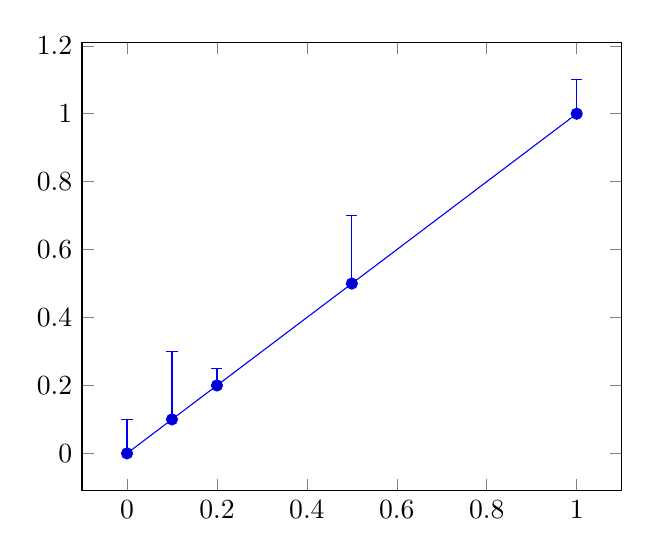
\begin{tikzpicture}
\begin{axis}
\addplot+[error bars/.cd,
	y dir=plus,y explicit]
coordinates {
	(0,0)     +- (0.5,0.1)
	(0.1,0.1) +- (0.05,0.2)
	(0.2,0.2) +- (0,0.05)
	(0.5,0.5) +- (0.1,0.2)
	(1,1)     +- (0.3,0.1)};
\end{axis}
\end{tikzpicture}
\end{codeexample}

The preceding example has two keys: |y dir=plus| configures \PGFPlots\ to \emph{activate} error bars for $y$ coordinates, but only upper bounds. The key |y explicit| tells \PGFPlots\ to expect \emph{absolute} values in the input data stream. In our case above, the input data stream is an |\addplot coordinates| which uses the special error--value--syntax |+- |$(\pgfplotserror{x}, \pgfplotserror{y})$, see the Section~\ref{sec:errorvalues:coords} for details.

It is allowed if the input data contains more error values than needed: our example above has error values for both $x$ and $y$ and it also contains lower bounds (since |+-| defines upper- and lower bounds simultaneously).

Consequently, the remaining values can be visualized as well:

\begin{codeexample}[]
\begin{tikzpicture}
\begin{axis}
\addplot+[error bars/.cd,
	y dir=both,y explicit,
	x dir=both,x explicit,
]
coordinates {
	(0,0)     +- (0.5,0.1)
	(0.1,0.1) +- (0.05,0.2)
	(0.2,0.2) +- (0,0.05)
	(0.5,0.5) +- (0.1,0.2)
	(1,1)     +- (0.3,0.1)};
\end{axis}
\end{tikzpicture}
\end{codeexample}

Error bars inherit all drawing options of the associated plot, but they use their own |error mark| and additional style arguments.

\begin{pgfplotsxykey}{error bars/\x\ dir=\mchoice{none,plus,minus,both} (initially none)}
	The initial configuration \declareandlabel{none} draws no error bars at all in the provided direction.

	The configuration \declareandlabel{plus} draws only upper bounds in the direction of interest.

	The configuration \declareandlabel{minus} draws only lower bounds in the direction of interest.

	The configuration \declareandlabel{both} draws upper and lower bounds in the direction of interest.

	In every case, the actual error value and its character (absolute or relative) is to be determined by other options (see below). If, for some reason, the error value is missing, the error bar is omitted.

\end{pgfplotsxykey}




\begin{pgfplotsxykey}{error bars/\x\ fixed=\marg{value} (initially 0)}
	Provides a common, absolute error $\pgfplotserror x=\text{\meta{value}}$ for all input coordinates.

\begin{codeexample}[]
\begin{tikzpicture}
\begin{axis}
\addplot+[error bars/.cd,
	y dir=both,y fixed=0.1,
]
coordinates {
	(0,0)
	(0.1,0.1)
	(0.2,0.2)
	(0.5,0.5)
	(1,1)
};
\end{axis}
\end{tikzpicture}
\end{codeexample}

	For linear $x$~axes, the error mark is drawn at $x \pm \pgfplotserror x$ while for logarithmic $x$~axes, it is drawn at $\log( x \pm \pgfplotserror x)$.
\end{pgfplotsxykey}

\begin{pgfplotsxykey}{error bars/\x\ fixed relative=\marg{percent} (initially 0)}
Provides a common, relative error $\pgfplotserror x = \text{\meta{percent}} \cdot x$ for all input coordinates. The argument \meta{percent} is thus given relatively to input $x$ coordinates such that $\text{\meta{percent}} = 1$ means $100\%$.

Error marks are thus placed at $x \cdot (1 \pm \pgfplotserror x)$ for linear axes and at $\log(x \cdot (1 \pm \pgfplotserror x))$ for logarithmic axes. Computations are performed in floating point for linear axis and using the identity $\log(x \cdot (1 \pm \pgfplotserror x)) = \log(x) + \log( 1 \pm \pgfplotserror x)$ for logarithmic scales.

The following example shows that fixed error values $\pgfplotserror{x}$ are independent of the input values.

\begin{codeexample}[]
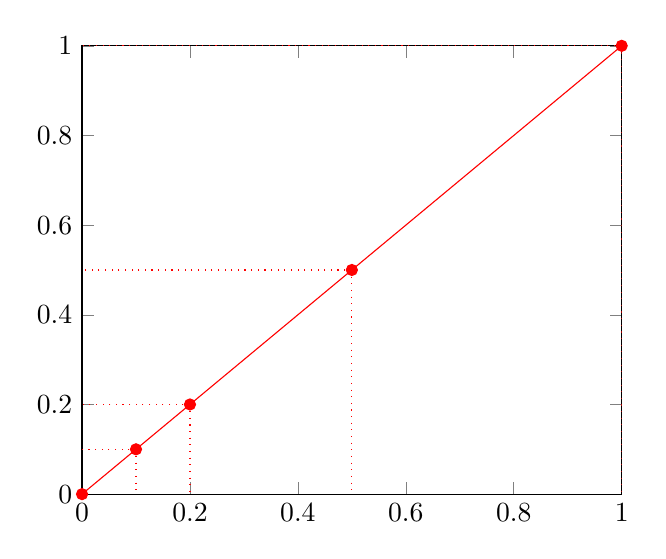
\begin{tikzpicture}
\begin{axis}[enlargelimits=false]
\addplot[red,mark=*]
	plot[error bars/.cd,
	y dir=minus,y fixed relative=1,
	x dir=minus,x fixed relative=1,
	error mark=none,
	error bar style={dotted}]
coordinates
	{(0,0) (0.1,0.1) (0.2,0.2) 	
	 (0.5,0.5) (1,1)};
\end{axis}
\end{tikzpicture}
\end{codeexample}
\end{pgfplotsxykey}

\begin{pgfplotsxykey}{error bars/\x\ explicit}
Configures the error bar algorithm to draw $x$-error bars at any input coordinate for which user-specified errors are available.
 Each error is interpreted as absolute error, see |x fixed| for details.

The different input formats of errors are described in Section~\ref{sec:errorbar:input}.
\end{pgfplotsxykey}

\begin{pgfplotsxykey}{error bars/\x\ explicit relative}
Configures the error bar algorithm to draw $x$-error bars at any input coordinate for which user-specified errors are available.
 Each error is interpreted as relative error, that means error marks are placed at $x (1 \pm \text{\meta{value}}(x))$ (works as for |error bars/x fixed relative|).
\begin{codeexample}[]
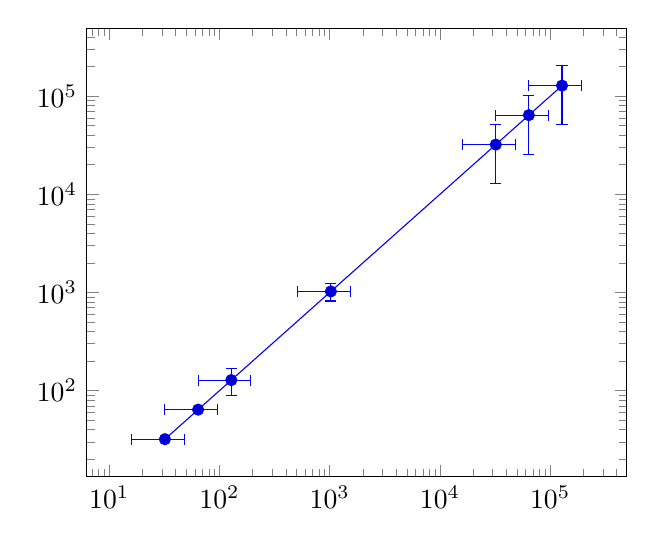
\begin{tikzpicture}
\begin{loglogaxis}
\addplot+[error bars/.cd,
	x dir=both,x fixed relative=0.5,
	y dir=both,y explicit relative,
]
table[x=x,y=y,y error=error]
{
    x       y       error
    32      32      0
    64      64      0
    128     128     0.3
    1024    1024    0.2
    32068   32068   0.6
    64000   64000   0.6
    128000  128000  0.6
};
\end{loglogaxis}
\end{tikzpicture}
\end{codeexample}

\end{pgfplotsxykey}


\begin{pgfplotskey}{error bars/error mark=\meta{marker}}
Sets an error marker for any error bar. \marg{marker} is expected to be a valid plot mark, see Section~\ref{sec:markers}.
\begin{codeexample}[]
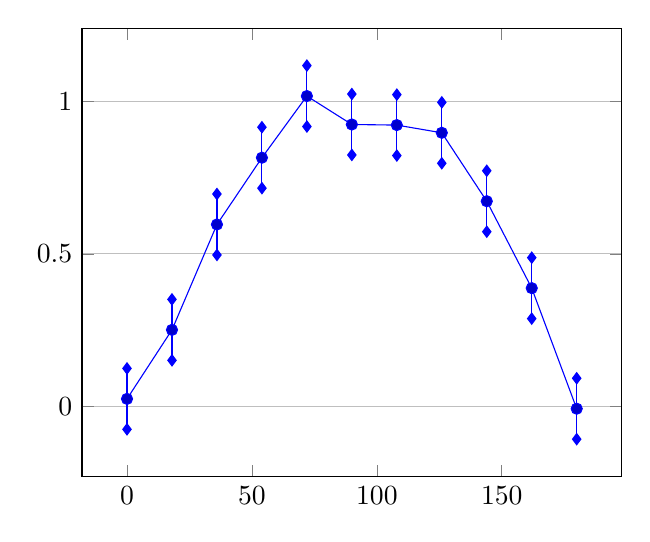
\begin{tikzpicture}
\pgfmathsetseed{42}
\begin{axis}[
	ymajorgrids,
]
\addplot+[
	domain=0:180,
	samples=11,
	error bars/.cd,
	y dir=both, y fixed=0.1,
	error mark=diamond*,
]
	{sin(x) + rand*0.1};
\end{axis}
\end{tikzpicture}
\end{codeexample}
\end{pgfplotskey}

\begin{pgfplotskey}{error bars/error mark options=\marg{key-value-list}}
Sets a key-value list of options for any error mark. This option works similarly to the \Tikz\ `|mark options|' key.
\end{pgfplotskey}

\begin{pgfplotskey}{error bars/error bar style=\marg{key-value-list}}
Appends the argument to `|/pgfplots/every error bar|' which is installed at the beginning of every error bar.
\end{pgfplotskey}

\begin{pgfplotscodetwokey}{error bars/draw error bar}
Allows to change the default drawing commands for error bars. The two arguments are
\begin{itemize}
\item the source point, $(x,y)$ and
\item the target point, $(\tilde x,\tilde y)$.
\end{itemize}
Both are determined by \PGFPlots\ according to the options described above. The default code is
\begin{codeexample}[code only]
\pgfplotsset{
	/pgfplots/error bars/draw error bar/.code 2 args={%
		\pgfkeysgetvalue{/pgfplots/error bars/error mark}%
			{\pgfplotserrorbarsmark}%
		\pgfkeysgetvalue{/pgfplots/error bars/error mark options}%
			{\pgfplotserrorbarsmarkopts}%
		\draw #1 -- #2 node[pos=1,sloped,allow upside down] {%
			\expandafter\tikz\expandafter[\pgfplotserrorbarsmarkopts]{%
				\expandafter\pgfuseplotmark\expandafter{\pgfplotserrorbarsmark}%
				\pgfusepath{stroke}}%
		};
	}
}
\end{codeexample}
\end{pgfplotscodetwokey}

\subsection{Input Formats of Error Coordinates}
\label{sec:errorbar:input}%
Error bars with explicit error estimations for single data points require some sort of input format. This applies to |error bars/x explicit| and |error bars/x explicit relative|.

\subsubsection{Error Coordinates and Coordinate Lists}
\label{sec:errorvalues:coords}
Error bar coordinates can be read from `|\addplot coordinates|' in which they are expected after data point as such:
\begin{codeexample}[code only]
\addplot coordinates {
	(1,2) +- (0.4,0.2)
	(2,4) +- (1,0)
	(3,5)
	(4,6) +- (0.3,0.001)
}
\end{codeexample}
where $(1,2) \pm (0.4,0.2)$ is the first coordinate, $(2,4) \pm (1,0)$ the second and so forth. The point $(3,5)$ has no error coordinate. The syntax \declareandlabel{+-} defines \emph{symmetric} error values, i.e.\ both upper and lower bound receive the same value.

Alternatively, one can use one of \declareandlabel{-=} and \declareandlabel{+=} to define asymmetric values:
\begin{codeexample}[]
\begin{tikzpicture}
\begin{axis}
\addplot+[
	error bars/.cd,
	x dir=both, x explicit,
	y dir=both, y explicit,
]
coordinates {
	(1.1,0.9) += (0.4,0.2) -= (0.1,0.1)
	(2.7,2) -= (1,0)
	(3,3)
	(3.8,4.2) +- (0.3,0.2)
};
\end{axis}
\end{tikzpicture}
\end{codeexample}
If multiple items (like multiple |+=|) for one coordinate are specified, the last one takes precedence.

Keep in mind that these error values are only displayed as error bars if |x dir| and |y dir| are set appropriately.

The input type |\addplot coordinates| also allows |point meta=explicit|, i.e.\ values of the form
\begin{codeexample}[code only]
\addplot coordinates {(0,0) [4]};
\end{codeexample}
This can be combined with error values. However, the point meta value in square brackets needs to be the last item:
\begin{codeexample}[code only]
\addplot coordinates {(0,0) +- (0.1,0.2) [4]};
\end{codeexample}


\subsubsection{Error Coordinates and Table Input}
The `|\addplot table|' format is
\begin{pgfplotsxykeylist}{%
	table/\x\ error=\marg{column name},
	table/\x\ error index=\marg{column index},
	table/\x\ error expr=\marg{math expression}}
	These keys define input sources for error bars with explicit error values.
	
	The |x error| method provides an input column name (or alias), the |x error index| method provides input column \emph{indices} and |x error expr| works just as |table/x expr|: it allows arbitrary mathematical expressions which may depend on any number of table columns using |\thisrow|\marg{col name}.

\begin{codeexample}[]
\begin{tikzpicture}
\begin{axis}
\addplot+[
	error bars/.cd,
	x dir=both, x explicit,
	y dir=both, y explicit,
]
table[y error=error]
{
	x   y   error
	1   0.9 0.4
	2   2.1 0.2
	3   3   0.1
	4   4.2 0.3
};
\end{axis}
\end{tikzpicture}
\end{codeexample}

In addition, one can provide column \emph{indices} using
\begin{codeexample}[code only]
\addplot table[x error index=COLINDEX,y error index=COLINDEX]
\end{codeexample}
These options are used like the `|x|' and `|x index|' options.

If you need to specify math expressions, you can use |x error expr|:
\begin{codeexample}[code only]
\addplot table[x error expr=\thisrow{errorx}^2]
\end{codeexample}
This is similar to |x expr|.
\end{pgfplotsxykeylist}

\begin{pgfplotsxykeylist}{%
	table/\x\ error plus=\marg{column name},
	table/\x\ error plus index=\marg{column index},
	table/\x\ error plus expr=\marg{math expression},
	table/\x\ error minus=\marg{column name},
	table/\x\ error minus index=\marg{column index},
	table/\x\ error minus expr=\marg{math expression}%
}
	These keys define input sources for error bars with \emph{asymmetric} error values, i.e.\ different values for upper and lower bounds.
	
	They are to be used in the same way as |x error|. In fact, |x error| is just a style which sets both |x error plus| and |x error minus| to the same value.

\begin{codeexample}[]
\begin{tikzpicture}
\begin{axis}
\addplot+[
	error bars/.cd,
	x dir=both, x explicit,
	y dir=both, y explicit,
]
	table[
		x error plus=ex+,
		x error minus=ex-,
		y error plus=ey+,
		y error minus=ey-,
	] {
	x   y   ex+   ey+  ex-  ey-
	1.1 0.9 0.4   0.2  0.1  0.1
	2.7 2   0     0    1    0
	3   3   0     0    0    0
	3.8 4.2 0.3   0.2  0.3  0.2
	};
\end{axis}
\end{tikzpicture}
\end{codeexample}
\end{pgfplotsxykeylist}

}%
